\documentclass[twocolumn]{article}
\usepackage[letterspace=-80]{microtype}
\usepackage{tikz}
\usetikzlibrary{shapes}
\usepackage{standalone}
\usepackage[includehead,includefoot,margin=1cm,headheight=1cm]{geometry}
\usepackage{stix2}
\usepackage{gillius}
\tikzset{>=stealth}
\usepackage{multicol}
\usepackage{environ}
\usepackage{lettrine}
\usepackage{mathtools}
\makeatletter
\newcommand{\mylabel}[2]{#2\def\@currentlabel{#2}\label{#1}}
\makeatother

\usepackage{qrcode}
\qrset{height=1cm}
\usepackage{fancyhdr}
\renewcommand{\headrulewidth}{0pt}
\fancypagestyle{title}{%
\fancyhead[L]{\sffamily\flushleft
\!\resizebox{!}{.05\textheight}{\documentclass{standalone}

\usepackage{tikz}

\begin{document}

\begin{tikzpicture}[x=1cm,y=1cm]
  \begin{scope}
    \clip(0,0) rectangle (73cm,12cm);
    %% X
    \begin{scope}[xshift=1cm]
    \draw[line width=2.5cm] (0,-2) -- (14,14);
    \draw[line width=2.5cm] (0,14) -- (14,-2);
    \end{scope}
    
    %% I
    \begin{scope}[xshift=16.5cm]
      \draw[line width=2.5cm] (0,0) -- (0,12);
    \end{scope}

    %% M
    \begin{scope}[xshift=19.5cm]
    \draw[line width=2.5cm, smooth, rounded corners=1cm]
    (0,0) -- (0,10.75)%% 
    --(3.5,10.75) % width of top
    --(6.5,1.25)--(8.5,1.25)
    --(11.5,10.75)
    --(15,10.75)--(15,0);
    \end{scope}

    %% E
    \begin{scope}[xshift=37.25cm,yshift=1.25cm]
      \draw[line width=2.5cm, smooth, rounded corners=2cm]
      (10,0)--(0,0)--(0,4.75)--(10,4.75);
      
      \draw[line width=2.5cm, smooth, rounded corners=2cm]
      (5,4.75) -- (0,4.75)--(0,9.5)--(11.8,9.5);
    \end{scope}

    %% R
    \begin{scope}[xshift=49cm,yshift=-1.25cm]
      \draw[line width=2.5cm, smooth, rounded corners=2cm]
      (0,12)--(10,12)--(10,7)--(0,7)--(0,1.25);
      
      \draw[line width=2.5cm]
      (4.5,7)--(10,0);
    \end{scope}

    %% A
    \begin{scope}[xshift=59.5cm,yshift=-1.25cm]
      \draw[line width=2.5cm, smooth, rounded corners=1.5cm]
      (0,0)--(6,12.75)--(12,0);
    \end{scope}
  \end{scope}
  %\draw[step=1cm,gray,very thin] (0,0) grid (71,10);
\end{tikzpicture}
\end{document}
}\resizebox{!}{.05\textheight}{\lsstyle
    Tech\! Brief}\\
Ximera: Interactive Mathematics Education  \\[-.1cm] Resources for All\hfill
\textsl{MathFest} 2024: August 7--9\\[.1cm]
\rule{\textwidth}{.1cm}\\[.1cm]\rmfamily
Email:~{\tt ximera@math.osu.edu} \hfill Website:~{\tt
https://github.com/ximeraProject/}}

\fancyfoot[L]{\sffamily\tiny\textbf{XIMERA\quad FORM \quad 1729 \quad GIT \quad
        COMMIT \quad
        \input{../.git/refs/heads/master} \quad PREVIOUS \quad EDITION \quad IS
        \quad OBSOLETE.}
}}

\fancypagestyle{main}{%
\fancyhead[L]{\sffamily\flushleft
\resizebox{!}{.7em}{\documentclass{standalone}

\usepackage{tikz}

\begin{document}

\begin{tikzpicture}[x=1cm,y=1cm]
  \begin{scope}
    \clip(0,0) rectangle (73cm,12cm);
    %% X
    \begin{scope}[xshift=1cm]
    \draw[line width=2.5cm] (0,-2) -- (14,14);
    \draw[line width=2.5cm] (0,14) -- (14,-2);
    \end{scope}
    
    %% I
    \begin{scope}[xshift=16.5cm]
      \draw[line width=2.5cm] (0,0) -- (0,12);
    \end{scope}

    %% M
    \begin{scope}[xshift=19.5cm]
    \draw[line width=2.5cm, smooth, rounded corners=1cm]
    (0,0) -- (0,10.75)%% 
    --(3.5,10.75) % width of top
    --(6.5,1.25)--(8.5,1.25)
    --(11.5,10.75)
    --(15,10.75)--(15,0);
    \end{scope}

    %% E
    \begin{scope}[xshift=37.25cm,yshift=1.25cm]
      \draw[line width=2.5cm, smooth, rounded corners=2cm]
      (10,0)--(0,0)--(0,4.75)--(10,4.75);
      
      \draw[line width=2.5cm, smooth, rounded corners=2cm]
      (5,4.75) -- (0,4.75)--(0,9.5)--(11.8,9.5);
    \end{scope}

    %% R
    \begin{scope}[xshift=49cm,yshift=-1.25cm]
      \draw[line width=2.5cm, smooth, rounded corners=2cm]
      (0,12)--(10,12)--(10,7)--(0,7)--(0,1.25);
      
      \draw[line width=2.5cm]
      (4.5,7)--(10,0);
    \end{scope}

    %% A
    \begin{scope}[xshift=59.5cm,yshift=-1.25cm]
      \draw[line width=2.5cm, smooth, rounded corners=1.5cm]
      (0,0)--(6,12.75)--(12,0);
    \end{scope}
  \end{scope}
  %\draw[step=1cm,gray,very thin] (0,0) grid (71,10);
\end{tikzpicture}
\end{document}
}\resizebox{!}{.7em}{\lsstyle
    Tech\! Brief}\hfill\textsl{MathFest} 2024: August 7--9\\[-.1cm]
\rule{\textwidth}{.1cm}\\[0cm]\rmfamily
Email:~{\tt ximera@math.osu.edu} \hfill Website:~{\tt
https://github.com/ximeraProject/}}

\fancyfoot[L]{\sffamily\tiny\textbf{XIMERA\quad FORM \quad 1729 \quad GIT \quad
        COMMIT \quad
        \input{../.git/refs/heads/master} \quad PREVIOUS \quad EDITION \quad IS
        \quad OBSOLETE.}}}

\usepackage[framemethod=TikZ]{mdframed}
\NewEnviron{xframe}{%
    \begin{mdframed}[roundcorner=2pt]
        \BODY%
    \end{mdframed}%
}

\begin{document}
\newgeometry{margin=1cm,headheight=3cm,includehead,includefoot}
\pagestyle{main}
\thispagestyle{title}
\pagenumbering{gobble}
\noindent
\lettrine[lines=2]{X}{imera}, pronounced ``chimera,'' is a free and
open-source platform offering tools for authoring and publishing
interactive educational content, including textbooks, assessments, and
online
courses. Currently, Ximera materials are utilized at over a dozen
institutions. \textbf{Even with the most conservative estimates, Ximera saves
    students
    over one million dollars annually}. The ultimate goal of this project is to
promote sustained student success and savings.

\begin{xframe}
    {\sffamily\bfseries Students} interact with \textit{content} produced
    within
    Ximera. Hence their experience is highly dependent on the
    \textit{quality} of
    the content itself. With that said, reseach \ref{F21} shows students in
    Ximera courses found the textbook to be more readable than a traditional
    course, and performed equivalently to students in courses that used
    propritory textbooks and online homework systems.
    While students typically learn about Ximera through their courses, many
    find Ximera content via web search and  use Ximera as independent learners.
    In 2023, we had over one million unique visitors to Ximera content. Since
    Ximera materials are free,
    anyone can access and use them, regardless of enrollment in official
    courses.
\end{xframe}

\begin{xframe}
    {\sffamily\bfseries Instructors} (who are not authors) can freely use
    any Ximera materials,
    \textbf{without permission}, by simply sharing the URLs of activites
    with their students. Many first time Ximera instructors start  by
    using online Ximera content as
    ungraded assignemnts. Visit our website for an incomplete list of
    Ximera courses that have been deployed online.
\end{xframe}

\begin{xframe}
    {\sffamily\bfseries Authors}  write and store their content on their own
    machines and GitHub repositories.
    Authors own their content and decide how to license their content. From a
    single source written in \LaTeX, Ximera generates various output: PDF
    worksheets,
    PDF textbooks, and	PDF solution manuals, and so on. Of most interest,
    Ximera can
    also create online interactive activities:
    \begin{center}
        \begin{tikzpicture}
            \node at (-1.8,.2)
            {\resizebox{.65cm}{!}{\documentclass[tikz]{standalone}
\begin{document}
\begin{tikzpicture}[rounded corners=.5pt]
\draw[fill=white] (0,0) -- (0,1.3) -- (.7,1.3) -- (1,1) -- (1,0) -- cycle;
\draw (.7,1.3) -- (.7,1) -- (1,1);
\end{tikzpicture}
\end{document}}};
            \node at (-1.8,.2) {\small PDF};
            \node at (-2,0) {\resizebox{.65cm}{!}{\documentclass[tikz]{standalone}
\begin{document}
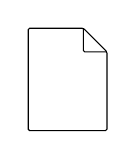
\begin{tikzpicture}[rounded corners=.5pt]
\draw[fill=white] (0,0) -- (0,1.3) -- (.7,1.3) -- (1,1) -- (1,0) -- cycle;
\draw (.7,1.3) -- (.7,1) -- (1,1);
\end{tikzpicture}
\end{document}}};
            \node at (-2,0) {\small PDF};
            \node at (-2.2,-.2)
            {\resizebox{.65cm}{!}{\documentclass[tikz]{standalone}
\begin{document}
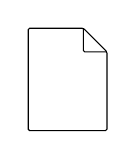
\begin{tikzpicture}[rounded corners=.5pt]
\draw[fill=white] (0,0) -- (0,1.3) -- (.7,1.3) -- (1,1) -- (1,0) -- cycle;
\draw (.7,1.3) -- (.7,1) -- (1,1);
\end{tikzpicture}
\end{document}}};
            \node at (-2.2,-.2) {\small PDF};
            \draw[->] (-.6,0) -- (-1.4,0);
            \draw[->] (-.6,.2) -- (-1.4,.2);
            \draw[->] (-.6,-.2) -- (-1.4,-.2);
            \node at (0,0) {\resizebox{1cm}{!}{\documentclass[tikz]{standalone}
\begin{document}
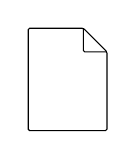
\begin{tikzpicture}[rounded corners=.5pt]
\draw[fill=white] (0,0) -- (0,1.3) -- (.7,1.3) -- (1,1) -- (1,0) -- cycle;
\draw (.7,1.3) -- (.7,1) -- (1,1);
\end{tikzpicture}
\end{document}}};
            \node at (0,0) {\LaTeX};
            \draw[->] (.6,0) -- (1.4,0);

            \node at (2,0) {\resizebox{1cm}{!}{\documentclass[tikz]{standalone}
\begin{document}
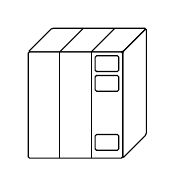
\begin{tikzpicture}[rounded corners=.5pt]
    \draw (0,0) rectangle (1.2,1.35);
    \draw (.4,0) -- (.4,1.35);
    \draw (.8,0) -- (.8,1.35);

    \draw (0,0)+(.85,1.1) rectangle ([shift={(.85, 1.1)}] .3, .2);
    \draw (0,0)+(.85,.85) rectangle ([shift={(.85, .85)}] .3, .2);
    \draw (0,0)+(.85,.1) rectangle ([shift={(.85, .1)}] .3, .2);

    \draw (1.2,0) -- (1.2,1.35) -- (1.5,1.65) -- (1.5,.3) -- cycle;

    \draw (0,1.35) -- (.3,1.65) -- (1.5,1.65) -- (1.2,1.35) -- cycle;
    \draw (.4,1.35) -- (.7,1.65);
    \draw (.8,1.35) -- (1.1,1.65);    
\end{tikzpicture}
\end{document}}};
            \draw[->] (2.6,0) -- (3.4,0);
            \node at (4,0) {\resizebox{1cm}{!}{\documentclass[tikz]{standalone}
\begin{document}
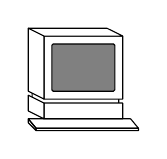
\begin{tikzpicture}[rounded corners=.1pt]
    \draw (-.15,-.1) rectangle (.95,.5);
    \draw[fill=white] (0,0) rectangle (1,.8);
    \draw[fill=white] (0,0) -- (-.2,.1) -- (-.2,.9) -- (.8,.9) -- (1,.8) -- (0,.8) --
    cycle;
    \draw (0,.8) -- (-.2,.9);
    \draw[fill=white] (0,-.05) -- (1,-.05) -- (1,-.25) -- (0,-.25) -- cycle;
    \draw[fill=white] (0,-.05) -- (0,-.25) -- (-.2,-.15) -- (-.2,.05) -- cycle;
    \draw[rounded corners=.5pt,fill=gray] (.1,.1) rectangle  (.9,.7);
    \draw (-.2,-.25) -- (1.1,-.25) -- (1.2,-.37) -- (-.1,-.37) -- cycle;
    \draw (-.2,-.25) -- (-.2,-.3) -- (-.1,-.4) -- (-.1,-.37) -- cycle;
    \draw (-.1,-.4) rectangle (1.2,-.37);
\end{tikzpicture}
\end{document}}};
            \node at (-2,-1) {Various};
            \node at (-2,-1.4) {PDFs};
            \node at (0,-1) {Single};
            \node at (0,-1.4) {Source};
            \node at (2,-1) {Deploy};
            \node at (2,-1.4) {Server};
            \node at (4,-1) {Students};
            \node at (4,-1.4) {Engage};

        \end{tikzpicture}
    \end{center}
    The source code used to produce a PDF produces an interactive online
    activity when deployed to  a Ximera server. Students access this content
    via a URL or an assignment in their
    LMS.
\end{xframe}

\begin{xframe}
    {\sffamily\bfseries Get involved} by contributing to the effort,
    either as an instrutor, an author, or a developer. Getting started with
    Ximera is
    easy---all you need is the XimeraLaTeX Package, available on CTAN. For more
    information, see our \textit{First Steps in Ximera} GitHub repository:
    \begin{center}
        \qrcode{https://go.osu.edu/xfs}\\
        \small\tt  https://go.osu.edu/xfs
    \end{center}
    As a token of our apprieciation and gratitude, please  consider applying for a \textbf{Ximera Flash-Grant Stipend} here:
    \begin{center}
        \qrcode{https://go.osu.edu/ximera-flash-grant}\\
        \small\tt  https://go.osu.edu/ximera-flash-grant
    \end{center}
    Thank you for your interest in Ximera. We encourage you to contact the team
    with  any questions you may have.
\end{xframe}

\begin{xframe}
    {\sffamily\bfseries Current development} is focused two critical
    aspects of Ximera: Streamlining the deployment
    process; Making LTI 1.3 support widely available.
    To this end, we are
    developing our
    deploy process using Docker and we are designing an assignment-grade
    database to
    seamlessly serve  learners at institutions supporting LTI 1.3, while also
    offering alternatives for self-learners and scenarios where
    LTI 1.3 is not available.
    \begin{center}
        \begin{tikzpicture}
            \node at (-3,1) [cloud, draw,cloud puffs=10,cloud puff arc=120,
                aspect=2, inner ysep=1em,scale=.8] {};
            \node at (-3,1) {LMS};
            \node at (-3,-1) {\resizebox{1cm}{!}{\documentclass[tikz]{standalone}
\begin{document}
\begin{tikzpicture}[rounded corners=.1pt]
    \draw (-.15,-.1) rectangle (.95,.5);
    \draw[fill=white] (0,0) rectangle (1,.8);
    \draw[fill=white] (0,0) -- (-.2,.1) -- (-.2,.9) -- (.8,.9) -- (1,.8) -- (0,.8) --
    cycle;
    \draw (0,.8) -- (-.2,.9);
    \draw[fill=white] (0,-.05) -- (1,-.05) -- (1,-.25) -- (0,-.25) -- cycle;
    \draw[fill=white] (0,-.05) -- (0,-.25) -- (-.2,-.15) -- (-.2,.05) -- cycle;
    \draw[rounded corners=.5pt,fill=gray] (.1,.1) rectangle  (.9,.7);
    \draw (-.2,-.25) -- (1.1,-.25) -- (1.2,-.37) -- (-.1,-.37) -- cycle;
    \draw (-.2,-.25) -- (-.2,-.3) -- (-.1,-.4) -- (-.1,-.37) -- cycle;
    \draw (-.1,-.4) rectangle (1.2,-.37);
\end{tikzpicture}
\end{document}}};
            \node at (-3,-2) {Students with LTI};
            \draw[->] (-3.1,-.4) -- (-3.1,.4);
            \draw[<-] (-2.9,-.4) -- (-2.9,.4);
            \node at (0,0) {\resizebox{1cm}{!}{\documentclass[tikz]{standalone}
\begin{document}
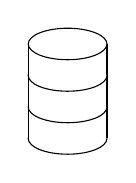
\begin{tikzpicture}[rounded corners=.5pt]
    \draw[fill=white] (.5,0) ellipse (.5cm and .2cm);  


    \draw[draw=none,fill=white] (0,0) rectangle (1,.4);
    \draw[] (0,0) -- (0,.4);
    \draw[] (1,0) -- (1,.4);    
    \draw[fill=white] (.5,.4) ellipse (.5cm and .2cm);  

    \draw[draw=none,fill=white] (0,.4) rectangle (1,.8);
    \draw[] (0,.4) -- (0,.8);
    \draw[] (1,.4) -- (1,.8);    
    \draw[fill=white] (.5,.8) ellipse (.5cm and .2cm);  


    \draw[draw=none,fill=white] (0,.8) rectangle (1,1.2);
    \draw[] (0,.8) -- (0,1.2);
    \draw[] (1,.8) -- (1,1.2);    
    \draw[fill=white] (.5,1.2) ellipse (.5cm and .2cm);  
\end{tikzpicture}
\end{document}}};
            \node at (0,-1) {Assignment};
            \node at (0,-1.4) {Database};
            \draw[->] (-2,.8) -- (-.6,.2);
            \draw[<-] (-2.1,.6) -- (-.7,0);
            \node at (3,-1) {\resizebox{1cm}{!}{\documentclass[tikz]{standalone}
\begin{document}
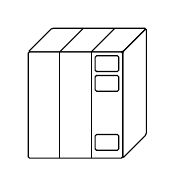
\begin{tikzpicture}[rounded corners=.5pt]
    \draw (0,0) rectangle (1.2,1.35);
    \draw (.4,0) -- (.4,1.35);
    \draw (.8,0) -- (.8,1.35);

    \draw (0,0)+(.85,1.1) rectangle ([shift={(.85, 1.1)}] .3, .2);
    \draw (0,0)+(.85,.85) rectangle ([shift={(.85, .85)}] .3, .2);
    \draw (0,0)+(.85,.1) rectangle ([shift={(.85, .1)}] .3, .2);

    \draw (1.2,0) -- (1.2,1.35) -- (1.5,1.65) -- (1.5,.3) -- cycle;

    \draw (0,1.35) -- (.3,1.65) -- (1.5,1.65) -- (1.2,1.35) -- cycle;
    \draw (.4,1.35) -- (.7,1.65);
    \draw (.8,1.35) -- (1.1,1.65);    
\end{tikzpicture}
\end{document}}};
            \node at (3,-2) {Deploy};
            \node at (3,-2.4) {Server};
            \node at (3,1) {\resizebox{1cm}{!}{\documentclass[tikz]{standalone}
\begin{document}
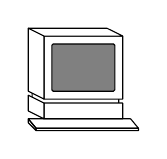
\begin{tikzpicture}[rounded corners=.1pt]
    \draw (-.15,-.1) rectangle (.95,.5);
    \draw[fill=white] (0,0) rectangle (1,.8);
    \draw[fill=white] (0,0) -- (-.2,.1) -- (-.2,.9) -- (.8,.9) -- (1,.8) -- (0,.8) --
    cycle;
    \draw (0,.8) -- (-.2,.9);
    \draw[fill=white] (0,-.05) -- (1,-.05) -- (1,-.25) -- (0,-.25) -- cycle;
    \draw[fill=white] (0,-.05) -- (0,-.25) -- (-.2,-.15) -- (-.2,.05) -- cycle;
    \draw[rounded corners=.5pt,fill=gray] (.1,.1) rectangle  (.9,.7);
    \draw (-.2,-.25) -- (1.1,-.25) -- (1.2,-.37) -- (-.1,-.37) -- cycle;
    \draw (-.2,-.25) -- (-.2,-.3) -- (-.1,-.4) -- (-.1,-.37) -- cycle;
    \draw (-.1,-.4) rectangle (1.2,-.37);
\end{tikzpicture}
\end{document}}};
            \node at (3,2) {Self-learner};
            \draw[->] (3.1,-.4) -- (3.1,.4);
            \draw[<-] (2.9,-.4) -- (2.9,.4);
            \draw[->] (2,.8) -- (.6,.2);
            \draw[<-] (2.1,.6) -- (.7,0);
            \draw[->] (2.3,-1) -- (.6,-.4);
            \draw[<-] (2.4,-.8) -- (.7,-.2);
        \end{tikzpicture}
    \end{center}

\end{xframe}

\begin{xframe}
    {\sffamily\bfseries Future development} will be directed toward making
    Ximera materials accessible to screen readers. This means navigating
    between activities in a document, navigating within an activity in the
    document, support for images and math, and support for our answer-box.
\end{xframe}
\restoregeometry

\begin{xframe}
    {\sffamily\bfseries Talks at \textsl{MathFest} featuring Ximera}
    \begin{itemize}
        \item[{[1]}] \textbf{Lines of Sight: Activities Related to Visual
            Perspective}. A.\ Davis; Thursday, August 8th,
        10:20am--10:35am,
        Room 309/310,
        \textit{New Twists on Your Favorite Math Circle Activity Part A}.
        \item[{[2]}] \textbf{Ximera in the Classroom}. B.\ Snapp and J.\
        Fowler;
        Friday, August 9th, 3:40pm--3:55pm, Room 313, \textit{Open-Source
            Products for
            the Advancement of Math Education Research and Practice}.
    \end{itemize}
\end{xframe}

\begin{xframe}
    {\sffamily\bfseries Reseach featuring Ximera}
    \begin{itemize}
        \item[\mylabel{F21}{[3]}] J.\ Fowler et al.\ \textit{An Open-Source
            Calculus
            Textbook on the Ximera Platform}. In:
        PRIMUS 31.9 (2021), pp.\ 925--939. %url: \texttt{https://doi.org/10.1080/10511970.2020.1781720}
        \item[{[4]}] E.\ Miller et al.\ \textit{Increasing active learning in
            large, tightly coordinated calculus courses}. In: Primus 31.3--5
        (2021), pp.\
        371--392.
        \item[{[5]}]S.D.\ Ryan \& T.M.\ Nawalaniec. \textit{An OER Approach to
            Linear Algebra}. In: PRIMUS 32.6 (2022), pp.\ 721--737.
        \item[{[6]}] P.\ Zachlin and A.\ Davis. \textit{A New Online
            Educational Resource (OER)
            for Linear Algebra}. In: MAA Focus 43.3 (2023), pp.\ 36--38.
    \end{itemize}
\end{xframe}

\begin{xframe}
    {\sffamily\bfseries Featured Ximera Activites}\hfill

    \def\arraystretch{4}%  1 is the default, change whatever you need
    \begin{tabular}{rl}
        \qrcode{https://go.osu.edu/lcis} &
        $\underset{\small\texttt{https://go.osu.edu/lcis}}{\textit{Lines and Curves in
        Space}}$                           \\
        \qrcode{https://go.osu.edu/mepr} &
        $\underset{\small\texttt{https://go.osu.edu/mepr}}{\textit{Systems: Number of
        Solutions (with Parameter)}}$      \\
        \qrcode{https://go.osu.edu/cfa}  &
        $\underset{\small\texttt{https://go.osu.edu/cfa}}{\textit{Comprehensive
        Factoring   Practice   Quiz}}$     \\
        \qrcode{https://go.osu.edu/met2} &
        $\underset{\small\texttt{https://go.osu.edu/met2}}{\textit{Math for Elementary
                    Teachers:	 Part II}}$
    \end{tabular}
\end{xframe}

\begin{xframe}
    \textbf{Funding for the Ximera Project} is provided by
    a U.S.\ Department of Education Open Textbooks Pilot Program grant in the
    amount of \$2,125,000, from 2024--2026, with no external funding. In the
    past, the Ximera Project has
    also recieved support from NSF Grant DUE-1245433, the Shuttleworth
    Foundation, the Ohio State University
    Department of Mathematics, and the Affordable Learning Exchange at OSU.
\end{xframe}

\end{document}
